\section{Podstawy teoretyczne}

  W dzisiejszych czasach sieci neuronowe zajmują ważną pozycję na rynku narzędzi
  do edycji obrazu. Jest to głównie spowodowane ich umiejętnością do
  reprodukowania i modelowania nieliniowych procesów, a także nowoczesnymi
  technikami przetwarzania plików graficznych.
  Jednak pierwsze architektury ANN (ang. artificial neural network) nie nadawały
  się do przetwarzania grafik.
  Było to częściwo spowodowane faktem, że obrazy, będące w rzeczywistości macierzami
  wartości pikseli,
  % należało przekształcić w długie wektory liczbowe aby móc podać je
  ciężko było skutecznie podać
  na wejscie typowych architekur DNN (ang. deep neural network) zbudowanych
  pierwotnie z wielu warst ukrytych, pomiędzy którymi połączenia są na zasadzie
  każdy z każdym oraz mają swoje wagi podlegające modyfikacji w trakcie procesu
  uczenia.
  Obrazy o niskiej rozdzielczości można było przekształcić w wektory
  wartości poszczególnych pikseli i w takiej postaci podawać na wejście sieci,
  jednak w przypadku obrazów o wyższej rozdzieloczości to rozwiązanie, ze
  względu na znaczną długość powstałych wektorów, nie oferowało dobrych
  rezultatów.
  Typowa stuktura DNN została przedstawiona na Rysunku \ref{fig:dnn}.
  Dopiero nowe architektury sieci spowodowały przełom w tej dziedzienie.

  \begin{figure}[h]
    \centering
    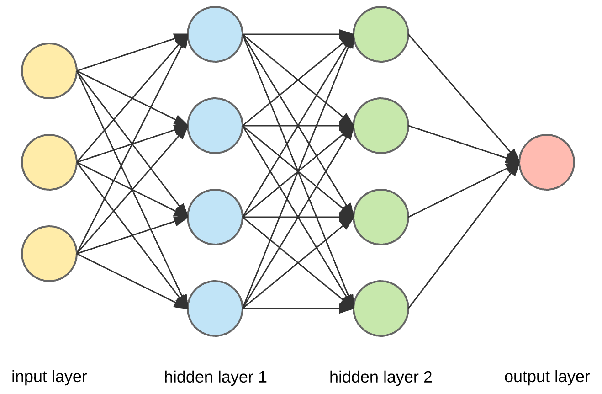
\includegraphics[width=4in]{dnn}
    \caption{Struktura DNN}
    \label{fig:dnn}
  \end{figure}

  Jedną z takich przełomowych architektur jest CNN (ang. convolutional neural
  network). Są to sieci o hierarchicznej strukturze, gdzie obrazy wejściowe w
  postaci macierzy wpier poddawane są ekstrakcji cech poprzez dokonanie operacji
  konwolucji na obrazie poprzez przesuwanie zestawu filtrów wzdłuż obrazu.
  Filtry te są zazywczaj inicjowane losowymi wartościami i w miarę trenowania,
  dopasowują swoje parametry do wybranej problematyki.
  Na wyjściu filtrów otrzymuje się macierze o mniejszej rozdzielczości
  reprezentujące wyniki operacji konwolucji w danym punkcie. Otrzymane macierze
  wyjściowe mogą być podawane na kolejne warstwy konwolucyjne w celu ekstrakcji
  kolejnych cech. Dzięki temu procesowi kolejne warstwy filtrów uczą się
  rozpoznawać kluczowe cechy na obrazie, od drobnych elemtów takich jak jak
  krawędzie albo kształty po bardziej złożone takie jak części ciała albo
  przedmioty.
  Końcowe warstwy dokonują spłaszczania, czyli zamieniania wielowymiarowych
  macierzy cech na jednowymiarowe wektore, które podawane są na wejście
  FCL (ang. fully connected layer).



  \subsection{Zastosowanie}

    \subsubsection{Alpha Zero}

    \subsubsection{Face App}

    \subsubsection{Chest radiograph classification}
